\chapter{Methodology}
\label{chap:methodology}

\section{Literature review}
\subsection{Run-of-the-river hydropower}
VGB Powertech defines a run-of-the-river hydropower plant as a hydropower plant that uses the natural usable stream without delaying it \cite{vgb}. \newline
Quaschning \cite{quaschning} describes how a run-of-the-river power plant operates.Even though there is no reservoir accumulating the water upstream from the plant, run-of-the-river power plants need an altitude difference, called head, between the water surface before and after the plant. This can be achieved through a dam, a derivation of the water stream through a canal, or a lock \cite{tdi_petites_centrales}. The water is lead through a turbine (see figure \ref{schema_hpp}) that drives a electrical generator, generating a power proportional to the water flow and the head, as seen in equation \ref{eq_power_1} \cite{quaschning}.
\begin{equation}
\label{eq_power_1} 
 P = \rho_\mathrm{water} \cdot g \cdot Q_\mathrm{turbine} \cdot H \cdot \eta_\mathrm{turbine} \cdot \eta_\mathrm{generator}
\end{equation}
With 
\begin{itemize}
\itemsep0em 
 \item $P$ \tabto{4cm} power produced by the generator \tabto{12cm} $[W]$
 \item $\rho_\mathrm{water}$ \tabto{4cm} density of water \tabto{12cm} $1000 \ kg/m^3$
 \item $g$ \tabto{4cm} acceleration of gravity \tabto{12cm} $9.81 \ m/s^2$
 \item $Q_\mathrm{turbine}$ \tabto{4cm} water flow through the turbine \tabto{12cm} $[m^3/s]$
 \item $H$ \tabto{4cm} head of water \tabto{12cm} $[m]$
 \item $\eta_\mathrm{turbine}$ \tabto{4cm} efficiency of the turbine
 \item $\eta_\mathrm{generator}$ \tabto{4cm} efficiency of the generator
\end{itemize}
\begin{figure}[H]
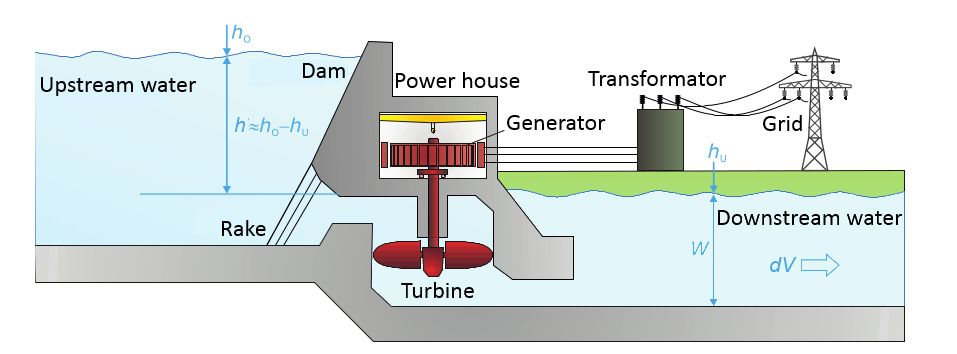
\includegraphics[width=15cm]{schema_hpp_en.png}
\caption[Schema of a run-of-the-river hydropower plant]{Schema of a run-of-the-river hydropower plant \cite{quaschning}}
\centering
\label{schema_hpp}
\end{figure}

The head of water is the altitude difference between the surface of the river before and after the turbine. For run-of-the-river hydropower plants, it is assumed that the water level before the turbine is kept constant by the dam, while the water level downstream can vary. This happens when the waterflow exceeds the capacity of the turbine and has to be deviated over the dam. With this assumption, the head of water is given by the equation \ref{eq_head} and the waterflow in the turbine by the equation \ref{eq_waterflow} \cite{quaschning}.
\begin{equation}
\label{eq_head} 
 H = H_\mathrm{n} +W_\mathrm{n}-W
\end{equation}
\begin{equation}
\label{eq_waterflow} 
 Q_\mathrm{turbine} = min(Q_\mathrm{n},Q)
\end{equation}
Where $H_\mathrm{n}$, $W_\mathrm{n}$ and $Q_\mathrm{n}$ are respectively the nominal head, water level downstream from the dam and water flow, and W and Q the real water level and water flow.
\newline
The  equation \ref{eq_power_1} becomes :
\begin{equation}
 \label{eq_power_2} 
 P = \rho_\mathrm{water} \cdot g \cdot min(Q_\mathrm{n},Q) \cdot (H_\mathrm{n} +W_\mathrm{n}-W) \cdot \eta_\mathrm{turbine} \cdot \eta_\mathrm{generator}
\end{equation}

The efficiency factor of the generator depends on its power and on the part-load range \cite{pacer}. The swiss ``Bundesamt für Konjunkturfragen'' gives the values given in table \ref{eta_gen}.

\begin{table}
 \caption[Generator efficiency in full load and part load]{Generator efficiency in full load (left) and part load (right) \cite{pacer}}
 \label{eta_gen}
 \begin{tabular}{|C{3cm}|C{3cm}| C{1cm} |C{3cm}|C{3cm}|}
  \cline{1-2} \cline{4-5}
  $P_\mathrm{el} [kW]$ & $\eta_\mathrm{g,max}$  && $P_\mathrm{el}/P_\mathrm{el, max}$ & $\eta_\mathrm{g}/\eta_\mathrm{g,max}$ \\ 
  \cline{1-2} \cline{4-5}
  1 to 5 & 80\% to 85\% && 
  \multirow{4}{*}{\begin{tabular}{c}>50\%\\25\% \\10\% \\\end{tabular}}& 
  \multirow{4}{*}{\begin{tabular}{c}100\% \\95\% \\85\% \\\end{tabular}}\\
  5 to 20 & 85\% to 90\% &&& \\
  20 to 100 & 90\% to 95\% &&&\\ 
  More than 100 & 95\% &&&\\ 
  \cline{1-2} \cline{4-5}
\end{tabular}
\end{table}

It is estimated that among the 6500 to 7500 hydropower plants in Germany, only 406 have a nominal power above 1MW \cite{uba_wasserkraft}. Out of 7500 run-of-the-river hydropower plants in the OpenEnergy Database, 5600 have a capacity under 100kW (see figure \ref{oedb_capa} in section \ref{hpp_register}).  However, the plants under 1MW account for a small part of the total installed power (see figure \ref{uba_hpp}). For that reason, the generator efficiency has been approximated to 95\% for all power plants is this work.

\begin{figure}[H]
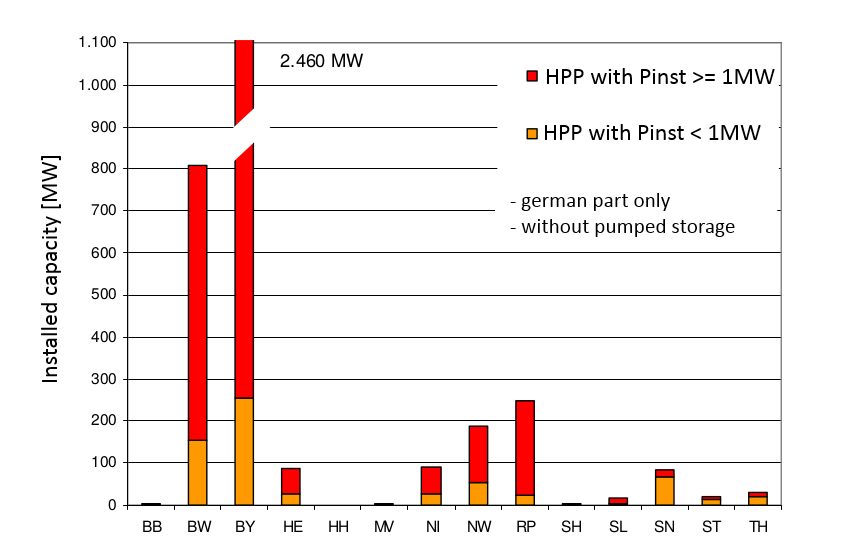
\includegraphics[width=15cm]{uba_hpp_en.png}
\caption[Installed power pro Bundesland for plants over and under 1MW]{Installed power pro Bundesland for plants over and under 1MW \cite{uba_wasserkraft}}
\centering
\label{uba_hpp}
\end{figure}

The efficiency of the turbine depends on the type of turbine and on the part-load range \cite{quaschning}\cite{pacer}. There are four types of turbines used for run-of-the-river plants : Pelton, Francis, Kaplan and crossflow. These turbines have optimal performances over ranges of water flow and hydraulic head, and their application areas can be plotted on a characterisitc diagramm, as in figure \ref{charac_diag}. XXX Add other Quelle in AnhangXXX

\begin{figure}[H]
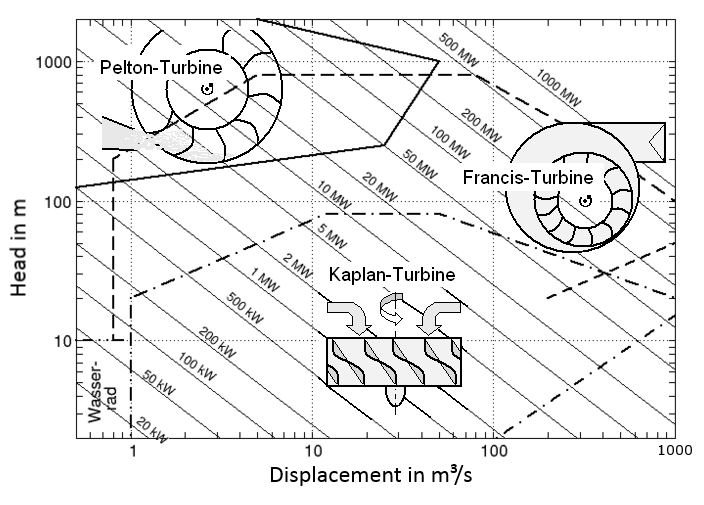
\includegraphics[width=14cm]{charac_diag_en.png}
\caption[Characteristic diagramm for several types of water turbines]{Characteristic diagramm for several types of water turbines \cite{wiki_WK}}
\centering
\label{charac_diag}
\end{figure}

Figure \ref{efficiency_turb} give the efficiency curves of different turbine types depending on the part load. These efficiencies can be approximated by the empiric function given in equation \ref{eq_eff} with the parameters given in table \ref{eff_param} \cite{quaschning}. In this equation, $Q_\mathrm{min}$ is the minimal water flow to start the turbine, $Q_\mathrm{n}$ is the nominal waterflow of the turbine and $q=\frac{Q-Q_\mathrm{min}}{Q_\mathrm{n}}$.

\begin{equation}
 \label{eq_eff}
\eta_\mathrm{T}= \left\{
    \begin{array}{ll}
	0 & \mbox{for } Q \leq Q_\mathrm{min}\\
        \frac{q}{a_\mathrm{1}+a_\mathrm{2} \cdot q + a_\mathrm{3} \cdot q^2} & \mbox{for } Q_\mathrm{min}<Q<Q_\mathrm{n} \\
        \eta_\mathrm{T,n} & \mbox{for } Q \geq Q_\mathrm{n}
    \end{array}
\right.
\end{equation}


\begin{figure}[H]
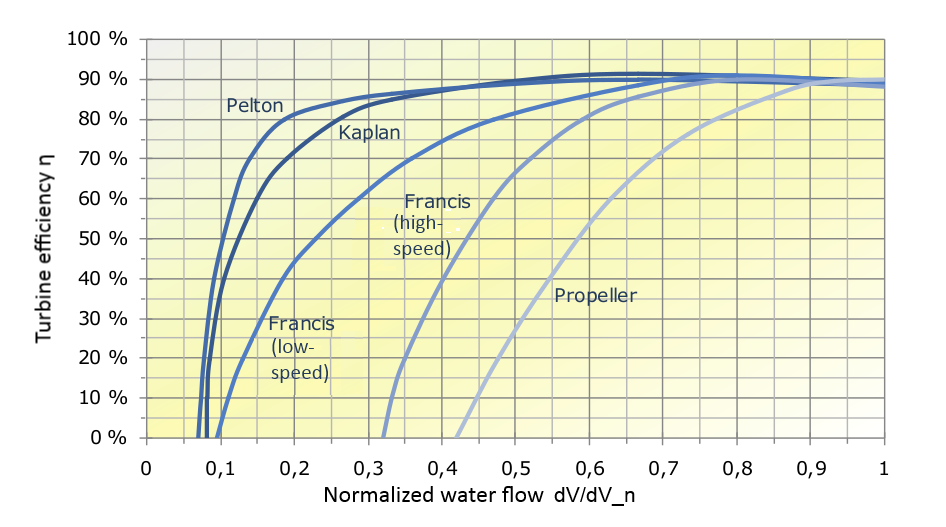
\includegraphics[width=15cm]{efficiency_turb_en.png}
\caption[Efficiency of different types of turbines depending on the part load ratio]{Efficiency of different types of turbines depending on the part load ratio (water flow / nominal water flow) \cite{raa89}}
\centering
\label{efficiency_turb}
\end{figure}


\begin{table}
 \caption[Parameters to calculate the turbine efficiency]{Parameters to calculate the turbine efficiency \cite{quaschning}}
 \label{eff_param}
 \centering
 \begin{tabular}{|c|c|c|c|c|c|}
  \cline{2-6}
  \multicolumn{1}{c|}{}&$Q_\mathrm{min} / Q\mathrm{n}$ & $\eta_\mathrm{T,n}$& $a_\mathrm{1}$ & $a_\mathrm{2}$&$a_\mathrm{3}$ \\ 
  \hline
  Kaplan & 0.081& 0.895& 0.045 &0.965& 0.1 \\
  Pelton & 0.07& 0.885& 0.03& 0.99& 0.1\\
  Francis &0.095 &0.89 &0.18 &0.63 &0.31 \\
  Propeller &0.42 &0.9 &0.25 &0.28 &0.69\\
  \hline
 \end{tabular}
\end{table}

\subsection{Related works}
Several works deal with the estimation of hydropower production. 
Several works use equation \ref{eq_power_1} or \ref{eq_power_2} to calculate the production or potential of run-of-river hydroelectricity on a given river \cite{hammid} \cite{bayazit} \cite{garrido}. In the case of potential assesment, the head of water can be obtained through geographic information systems (GIS) by calculating the elevation difference between neighbouring cells. The runoff can also be assessed from weather data using GIS, as described by Döll in figure \ref{waterGAP}.


Gesine usw

\section{Available data}

\subsection{Hydropower plants registers and data about hydropower}
\label{hpp_register}

This work, as well as the project open\_FRED, is linked to the OpenEnergy Platform, developped by the Reiner Lemoine Institute within the open\_eGo project. The OpenEnergy Platform provides necessary tools for transparent and collaborative energy system modeling \cite{oedb}, such as grid data, power plants register, geography data or weather data. The OpenEnergy Database has 7491 entries for run-of-the-river hydropower plants in Germany and contains (among others) the following information :
\begin{itemize}
\itemsep0em 
 \item EEG ID
 \item Company operating the plant
 \item Adress and state
 \item Startup, retrofit and shutdown years
 \item Electrical capacity [MW]
 \item Network operator information
 \item Position (latitude, longitude, and GIS geometry)
\end{itemize}


Figure \ref{oedb_capa} shows the repartition of the capacity of these plants. This is consistent with the Umweltbundesamt numbers of 6500 to 7500 hydropower plants excluding pumped hydro, among which 406 with a nominal power above 1MW \cite{uba_wasserkraft}. 

\begin{figure}[H]
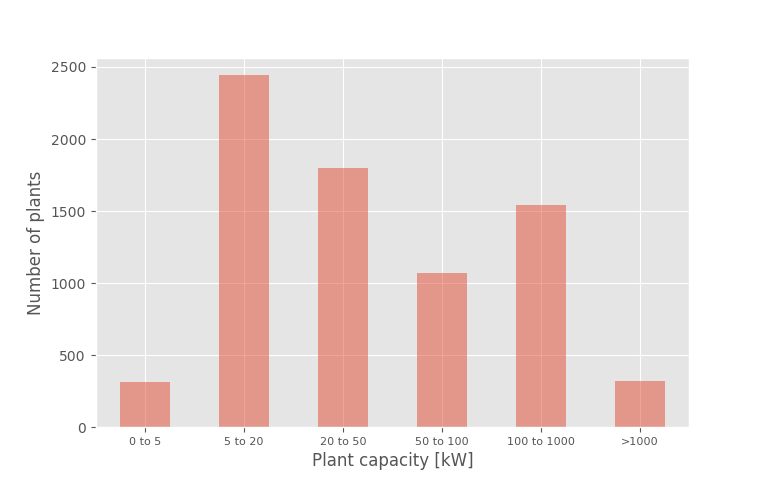
\includegraphics[width=15cm]{oedb_capa.png}
\caption[Repartition of the capacity of hydropower plants in the OpenEnergy Database]{Repartition of the capacity of hydropower plants in the OpenEnergy Database - own representation}
\centering
\label{oedb_capa}
\end{figure}


The Agentur für Erneuerbare Energien (AEE) provides data about the installed capacity, electricity generation over the year and number of hydropower plants for each Bundesland \cite{aee} from 2001 to 2014 (based on data from the Bundesverband der Energie- und Wasserwirtschaft). However, this data is for hydropower in general, including reservoir plants and pumped hydro, and might show discrepancies with the OEDB database. Table \ref{oedb_aee_diff} lists the number of plants and installed capacity per Bundesland from these two sources, as well as the relative difference for each state, with the AEE data as reference.  

\begin{table}
\footnotesize 
 \caption[Number of hydropowerplants and installed capacity per Bundesland]{Number of hydropowerplants and installed capacity per Bundesland \cite{oedb}\cite{aee}}
 \centering
 \label{oedb_aee_diff}
 \begin{tabular}{|c|cc|cc| cc|}
  \cline{2-7}
  \multicolumn{0}{c|}{} &\multicolumn{2}{|c}{\textbf{OEDB}}&\multicolumn{2}{|c|}{\textbf{AEE}}&\multicolumn{2}{c|}{\textbf{Difference}} \\
  \hline
  \textbf{State} & Number 	& 	Capacity [MW] 	&	Number 	& 	Capacity [MW] 	&	Number [\%] 	&	Capacity [\%] \\
  \hline
  SH	&	29	&	8.1		&	24	&	5		&	20.8		&	62.8	\\
  HH	&	1	&	0.11		&	1	&	0.1		&	0		&	10	\\
  NI	&	258	&	56.3		&	257	&	70		&	0.4		&	-19	\\
  HB	&	1	&	10		&	1	&	10		&	0		&	0	\\
  NRW	&	437	&	137.8		&	409	&	202		&	6.9		&	-31.8	\\
  HE	&	463	&	51.9		&	482	&	82		&	-3.9		&	-36.7	\\
  RLP	&	217	&	40.8		&	199	&	218		&	9		&	-81.3	\\
  BW	&	1741	&	464.5		&	1485	&	960		&	17		&	-51.6	\\	
  BY	&	3657	&	666.2		&	3578	&	2661		&	2.2		&	-75	\\
  SL	&	26	&	11.1		&	26	&	24		&	0		&	-53.6	\\
  B	&	0	&	0		&	0	&	0		&	0		&	0	\\
  BB	&	42	&	5.3		&	38	&	6		&	10.5		&	-11.8	\\
  MV	&	25	&	3		&	24	&	3		&	4.2		&	-0.1	\\
  SN	&	322	&	134.4		&	330	&	99		&	-2.4		&	35.8	\\
  ST	&	57	&	26		&	52	&	26		&	9.6		&	0.2	\\
  TH	&	204	&	32.6		&	198	&	32		&	3		&	2	\\
  \hline
 \end{tabular} 
\end{table}

The relative difference is shown on maps \ref{map_diff_num} and \ref{map_diff_pow}, which respectively display the differences in the number of plants and in the installed capacity. The analysis of these two maps and of table \ref{oedb_aee_diff} shows that the OEDB and AEE databases are consistant in three federal state : Thuringia, Saxony-Anhalt and Mecklenburg-Vorpommern (Berlin and Bremen being excluded due to the near absence of hydropower). The discrepencies in other federal states can be explained by different reasons. First, the data of the the AEE are based on all hydropower plants, including reservoir plants. This is why both the number of plants and the installed capacity are greater in the AEE data for most states. Second,these reservoir plants tend to have a bigger capacity than most run-of-the-river plants, which explains that the difference in installed capacity is not proportionnal to the difference in number of plants. Finally, rivers often mark boundaries between states and countries, and some hydropower plant are operated by two countries or inject electricity into the grids of more than one country. It is possible that the AEE and the OEDB don't count the installed capacity in the same manner in this situation. Map \ref{map_diff_pow} shows a bigger discrepency in installed capacity for border states.
\newline
For this reason, the state-wide simulation of hydropower production presented in the case study from section XXX UPDATE WHEN READY XXX as been conducted for XXX TH or ST or MV XXX, in order to compare the results of the simulation based on the OEDB register with the yearly production values given by the AEE.

\begin{figure}[H]
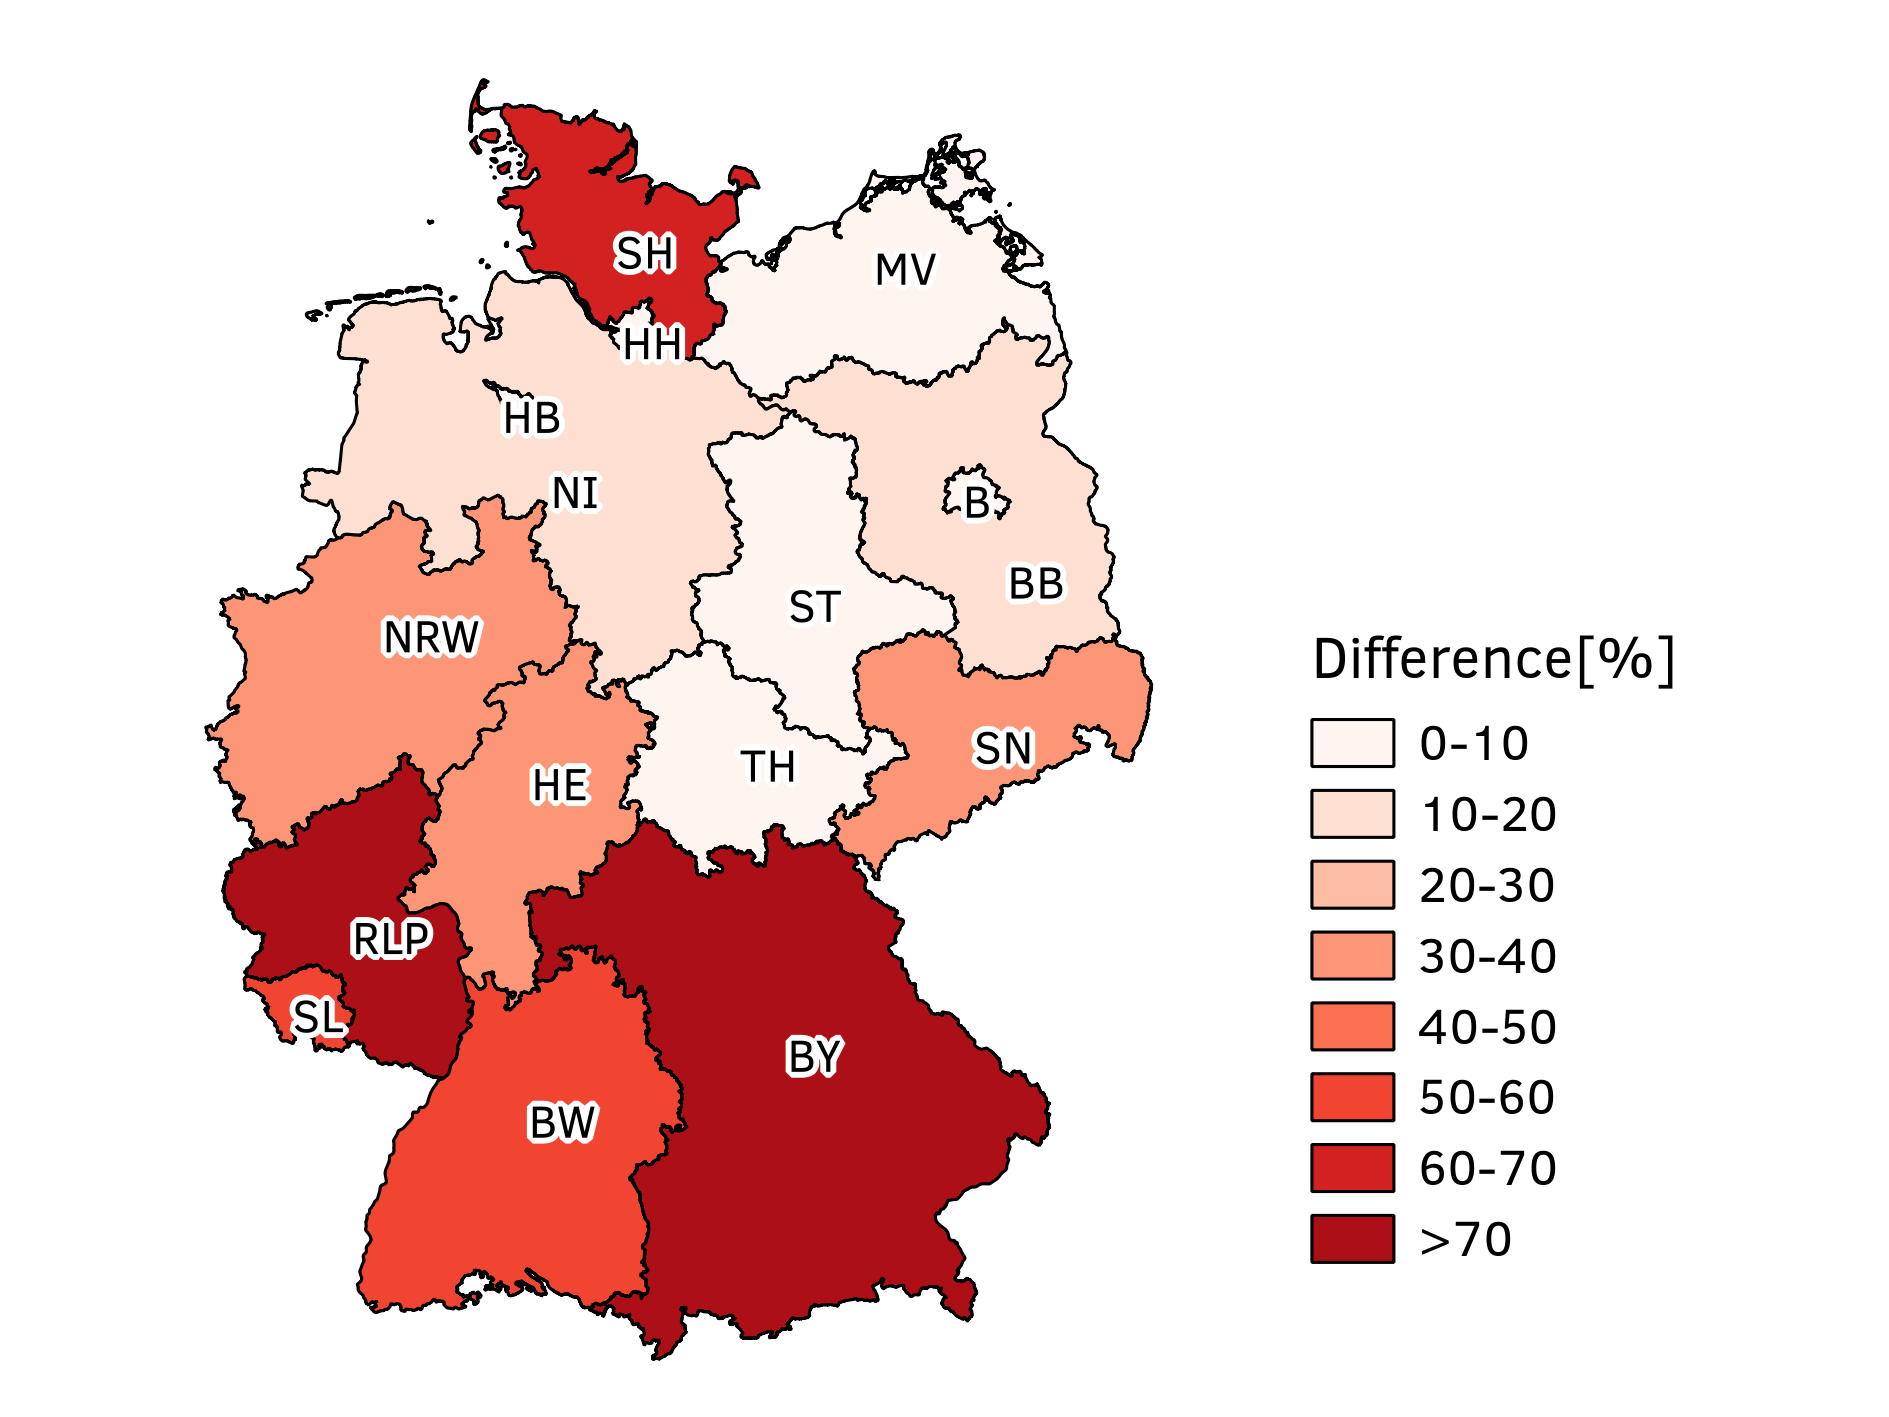
\includegraphics[width=15cm]{map_diff_pow.png}
\caption[Repartition of the ROR plant capacities in the open energy database]{Repartition of the plant capacities in the open energy database - own representation}
\centering
\label{map_diff_pow}
\end{figure}


\begin{figure}[H]
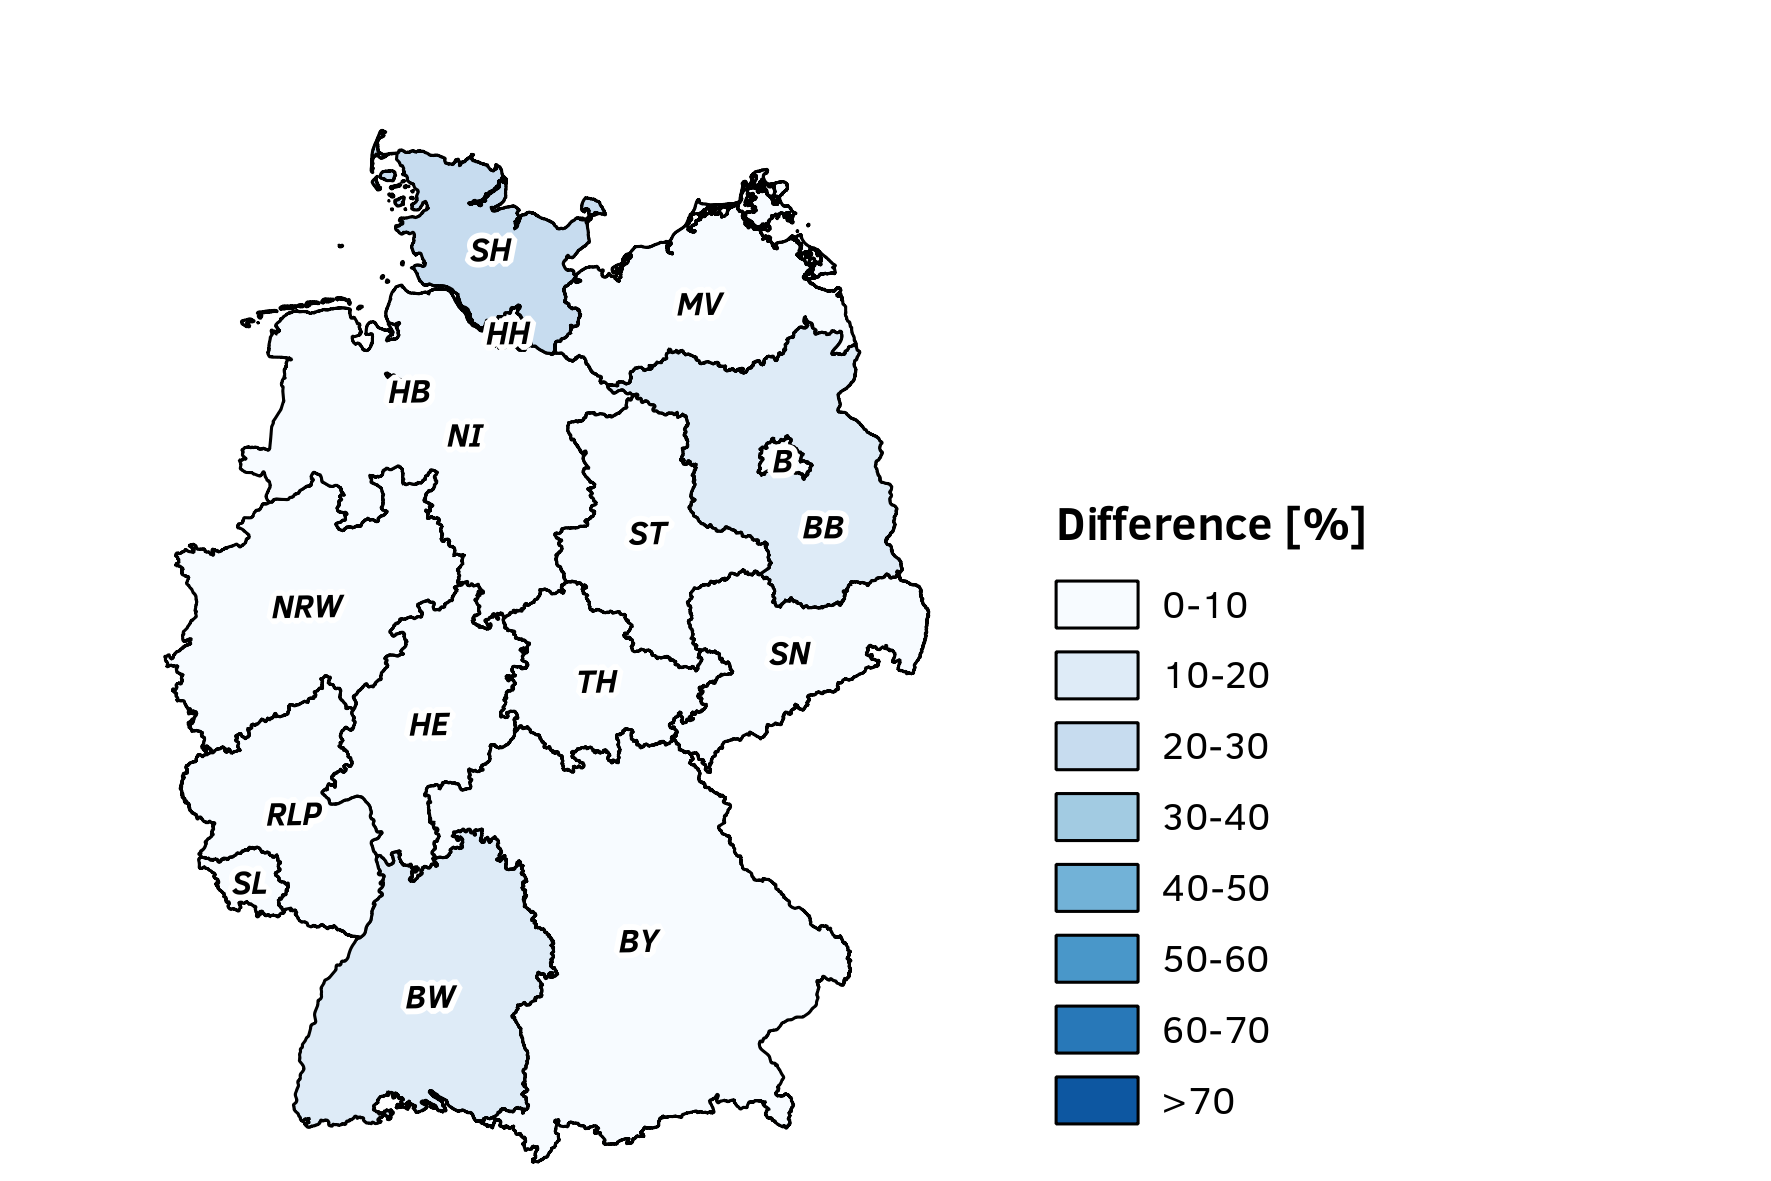
\includegraphics[width=15cm]{map_diff_num.png}
\caption[Repartition of the installed capacity per Bundesland (OEDB data)]{Repartition of the installed capacity per Bundesland (OEDB data)- own representation}
\centering
\label{map_diff_num}
\end{figure}


\subsection{Modeling runoff}
Modelling runoff is a difficult task, as the model has to assess the interactions between river sources, relief, rainfall, local soil and vegetation type, as well as anthropogenic use. This can be done using GIS \cite{bayazit}, by assigning each cell with the precedent parameters. The water input in each cell (rainfall, water sources and runoff from other cells) is converted in runoff from the cell by subtracting the water lost by infiltration, evapotranspiration, or anthropogenic use, and the runoff direction is given by the slope, calculated using a digital elevation model \cite{heywood}. \newline
The waterGAP software, developed by the universities of Kassel and Frankfurt, uses this method to calculate flows and storages of water around the globe, as shown on figure \ref{waterGAP}.

\begin{figure}[H]
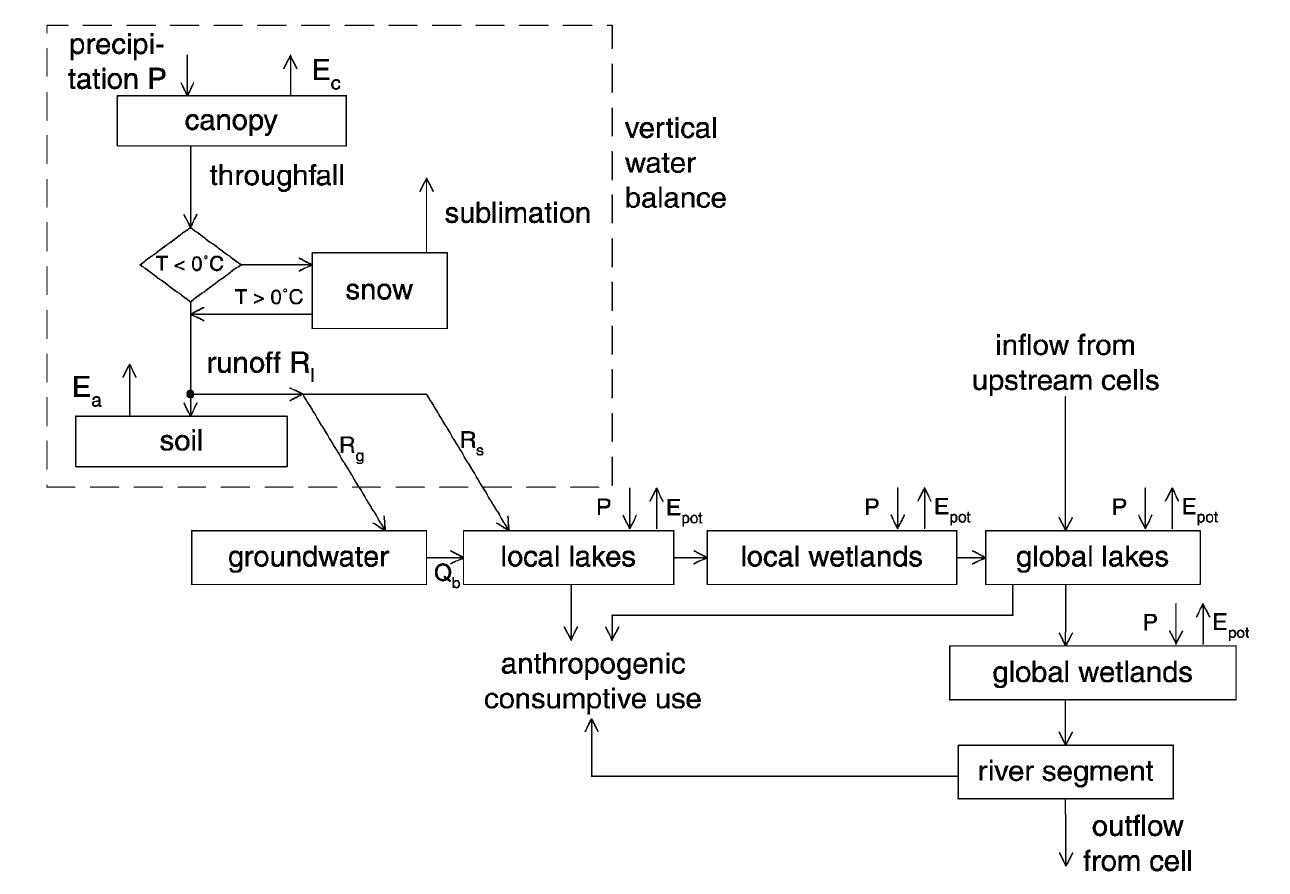
\includegraphics[width=15cm]{waterGAP.png}
\caption[Representation of a global hydrological from the WaterGAP software]{Representation of a global hydrological from the WaterGAP software \cite{doll}}
\centering
\label{waterGAP}
\end{figure}

Given that this work is part of the openFRED project (see introduction) the runoff data should eventually be accessible from open source databases or software. A model is currently being developed by the Helmholtz Zentrum Geesthacht in partnership with the Reiner Lemoine Institute, in order to be used in the openFRED project. This model was not yet available during this work, therefore other sources where used for runoff data (see section \ref{meas_runoff}).

\subsection{Measured runoff}
\label{meas_runoff}
Water levels and water flows of the main rivers are regularly measured and documented by several organizations, in order to keep track of the history of the waterways and to anticipate potential floods. In Germany, the German Federal Institute of Hydrology (Bundesanstalt für Gewässerkunde – BfG), is a supreme federal agency within the portfolio of the Federal Ministry of Transport and Digital Infrastructure. As such it is the federal government's scientific institution for research, assessments, and consulting in the fields of hydrology, uses, quality and conservation of waters and ecology \cite{bafg}. The BfG gathers data about water levels and water flows since its founding in 1949 and publishes it every year in the ``Deutsches Gewässerkundliches Jahrbuch'' (DGJ). The BfG also operates the HYDABA database, in which times series for water flow and water level are stored, going back to 1816 for daily values and 1981 for hourly values. This database gathers water levels from around 600 gauges and water flows from around 250 stations. The data can, among others, be provided to universities, public administrations, engineering or insurance companies \cite{bafg_hyd}. \newline
Another source of measured river data is Pegelonline, a service of the Federal Waterways and Shipping Administration (WSV). It publishes raw values of water levels from around 600 gauges in Germany over the previous 30 days. Some of the stations also measure water flows \cite{pegelonline}. The locations of the gauges are shown on map \ref{pegelonline}.

\begin{figure}[H]
\centering
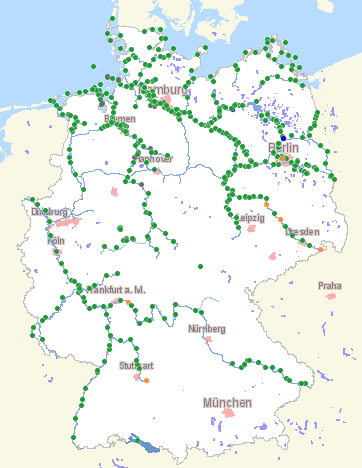
\includegraphics[width=8cm]{pegelonline.png}
\caption[Locations of the gauge stations]{Locations of the gauge stations \cite{pegelonline}}
\label{pegelonline}
\end{figure}

In this work, data from the BfG was used as input to test the model (XXX put references of teil über Mosel und Thuringe XXX), as well as data from the french ``Banque Hydro'' (XXX reference of the teil über Hydroraon XXX). The ``Banque Hydro'' is run by the SCHAPI (Service Central d'Hydrométéorologie et d'Appui à la Prévision des Inondations), a section of the french Ministry of Ecology, Sustainable Development and Energy, and gathers data from around 5000 gauge stations.

\section{Specifications of the model}

\subsection{Inputs and outputs}
\label{in_out}

In order to predict with precision the electrical output of a run-of-the-river power plant, the following parameters and values would be needed : 
\begin{itemize}
\itemsep0em
 \item Power plant parameters : 
 \begin{itemize}
  \item nominal water flow through the turbine ($Q_\mathrm{nenn}$)
  \item nominal head of water ($H_\mathrm{nenn}$)
  \item nominal water level ($W_\mathrm{nenn}$)
  \item efficiency curve of the turbine ($\eta_\mathrm{turbine}$) 
  \item efficiency of the generator ($\eta_\mathrm{generator}$)  
  \item unusable water flow ($Q_\mathrm{rest}$)  
 \end{itemize}
 \item Input time series : 
 \begin{itemize}
  \item actual water flow through the turbine ($Q$)
  \item actual water level downstream from the turbine ($W$)
 \end{itemize}
\end{itemize}

However, if such precise data can be found for single power plants, it is not easily accessible at a state or country-wide level. The OEDB database lists the location and nominal power of the plants, without further information on their design. The german Bundesnetzagentur is developing a register of every energy production facility in Germany, called MaStR (Marktstammdatenregister). This register should give a complete overview of the power plants in Germany, sorted by energy carrier and type of plant (reservoir, run-of-the-river, pumped hydro...), and listing the location and nominal power, as well as the presence or not of a restriction of the usable water flow due to a fish ladder or fish protection system for instance \cite{MaStR}. This last information is not yet available in registers such as the OEDB.\newline
Therefore, the model should be able to extrapolate missing data and to make some assumptions when optional input parameters are not provided. The only compulsory input parameter will be the broadly available nominal power of the turbine and section \ref{missing_data} explains how other parameters can be assumed or extrapolated. \newline
In terms of time series, in addition to the water flow over the simulated period, the model will take as input the water flow over several years in order to extrapolate missing parameters. Section \ref{rel_river_data} will go more in details into the reasons why water level data is not relevant. \\
The desired outputs for the model are electricity production time series per power plant or per area. It should also be possible to simulate several plants in one go.


\subsection{Tools}

In order to fulfill the specifications listed in section \ref{in_out}, several computational tools are necessary. The model itself is written in Python, an interpreted programming language, and linked to the OpenEnergy Database, where the input data are stored and accessed by SQL queries. The model is accessible on Github under https://github.com/hydro-python/hydropowerlib/
Furthermore, QGIS, a geographic information software, was used to assign rivers and gauge stations to the hydropower plants of the OpenEnergy Database. This is detailed in section \ref{assign_rivers}. Image XXX DO A GRAPH OF INTERACTIONS BETWEEN TOOLS XXX shows the interactions between the different tools.
